 %%%%%%%%%%%%%%%%%%%%%%%%% CHAPTER %%%%%%%%%%%%%%%%%%%%%%%%%%%%%%%%
\chapter{Redes Neuronales Convolucionales}


Las primeras Redes Neuronales Convolucionales (CNN por sus siglas en inglés) datan de 1980  por Fuksihima \cite{firstCnn} y 1998 desarrollada por Yann Lecun \cite{lecunCnn}. Sin embargo, no fue hasta el 2012 con la introducción de la AlexNet \cite{alexnet} que la comunidad científica empezó a destinar recursos considerables a su estudio. Con el propósito de entender a profundidad a las CNNs, definiremos lo que es una convolución. Para un estudio más detallado es posible consultar \cite{CNNdefinition,deeplearningbook}. 

%------------------------------ 1.Convoluciones -----------------------
\section{Convoluciones}
La convolución es una operación binaria que tiene muchas aplicaciones en los campos de matemáticas y física \cite{convolution_for_quaternion}, tales como álgebra lineal y procesamiento de señales. En cuánto a Inteligencia Artificial se refiere, las convoluciones son utilizadas para construir arquitecturas invariantes ante las traslaciones \cite{convolution_invariance}. A continuación se definen matemáticamente las convoluciones y en la Sección \ref{section_cnn} se definen las CNNs.
 \begin{definition}[Convolución]
    \label{convolution_definition}
     Sean $f,g : \R \to \R$. La convolución de $f$ con $g$, denotada como $f * g$ se define como:
     $$(f*g)(t) = \int_{0}^t f(\tau)g(t-\tau)d\tau$$
 \end{definition}

 Uno de las propiedades de las convoluciones es que son invariantes ante las traslaciones \cite{convolution_invariance}.
\begin{proposition}
    Sea $T_af$ el operador de traslación definido por $T_af(t) = f(t+a)$. Se tiene que 
    \begin{equation}
        T_a(I*K) = (T_af)*K.
    \end{equation}
\end{proposition}

 Sin embargo la Definición \ref{convolution_definition} no es muy práctica para los paradigmas computacionales, pues  las limitaciones físicas nos obligan discretizar la integral a modo de suma. Además, las imágenes son funciones cuyo dominio es subconjunto de $\mathbb R^2$. Por lo que es necesario extender la definición \ref{convolution_definition} a más de una dimensión.
 \begin{definition}[Convolución de una imagen con un kernel]
     Sea $I$ una imagen y $K$ un kernel bidimensional. La convolución de $I$ con $K$ es la imagen $(I*K)$ definida como:
     $$(I*K)(i,j) = \sum_m\sum_n I(m,n)K(i-m,j-n).$$ 
 \end{definition}
 En varias bibliotecas de aprendizaje automático se implementa una correlación cruzada en lugar de una convolución. La única diferencia entre una correlación cruzada y una convolución es la orientación del Kernel. En este trabajo, adoptaremos la convención usual de referirnos a las correlaciones como convoluciones. 
 \begin{definition}
     Sea $I$ una imagen y $K$ un kernel bidimensional. La correlación cruzada de $I$ con $K$ es la imagen definida por 
     $$(I*K)(i,j) = \sum_m\sum_n I(i+m,j+n)K(m,n).$$ 
 \end{definition} 

 \begin{figure}[H]
     \centering
     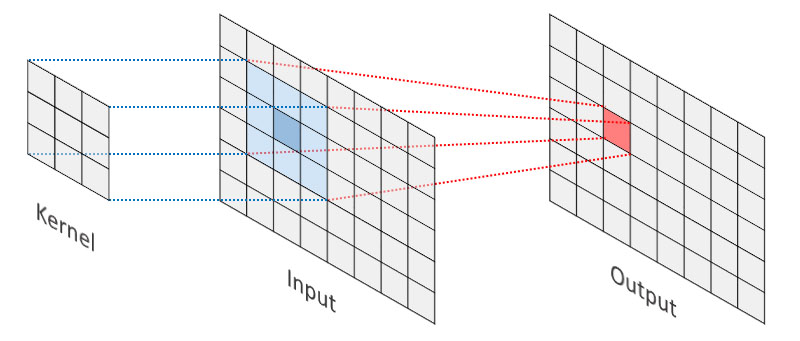
\includegraphics[width=4in]{../src/ch1convolution.png}
     \caption{Representación gráfica de una convolución. Para cada posición del Kernel sobre la imagen, se realiza una multiplicación \textsl{entrada por entrada} del Kernel y la un conjunto de pixeles de la imagen, del mismo tamaño que el Kernel.} 
 \end{figure}
 Cuando calculamos la correlación cruzada, desplazamos el kernel 1 pixel a la vez. Sin embargo, es posible aumentar la cantidad de pixeles que avanza el kernel en cada iteración. A esto se le conoce como tamaño de paso 

 
 %------------------------------ Stride -----------------------
 \subsection{Stride}
 \begin{definition}
    Sea $x$ una característica, y $K$ un kernel. Denotamos la correlación cruzada con tamaño de paso $a$, de la siguiente manera 
    \begin{equation}
        (I*K)|_a = (I*K)(i,j) = \sum_m\sum_n I(i+m+a \cdot i,j+n+a \cdot j)K(m,n)
    \end{equation}
 \end{definition}
 Debido a lass convenciones en la notación, a la correlación cruzada con tamaño de paso $a$, también se le llamará \textsl{convolución con tamaño de paso $a$}.

 \begin{figure}[H]
    \centering
    \includegraphics[width=4in]{../cap2_CNNs/src/stride_convolution.png}
    \caption{Convolución con tamaño de paso 2} 
\end{figure}
 %------------------------------ Convoluciones con múltiples canales -----------------------
 \subsection{Convoluciones con múltiples canales}
 Las imágenes RGB suelen tener 3 canales, cada uno representa la intensidad de cada color: rojo, verde y azul respectivamente. Más aún, en las redes modernas, se suelen hallar características con múltiples canales, en cada capa. Es por esto, que es imperativo definir convoluciones para características con más de un canal.
 Antes de definir lo que es una convolución para múltiples canales, definiremos un concepto más general de \textsl{kernel}.
 \begin{definition}
    Decimos que un kernel $K$ multicanal tiene $d_1$ canales de entrada y $d_2$ canales de salida cuando $K\in \mathbb R^{k\times k\times d_1 \times d_2}$.
    $$K = \left(
        \begin{matrix}
            K_{1,1} & K_{1,2} & \cdots & K_{1,d_2} \\
            K_{2,1} & K_{2,2} & \cdots & K_{2,d_2} \\
            \vdots & \vdots & \ddots & \vdots \\
            K_{d_1,1} & K_{d_1,2} & \cdots & K_{d_1,d_2} \\
        \end{matrix}
    \right)$$  
    Cada $K_{i,j}\in \mathbb R^{k\times k}$ representa un subfiltro de $K$.
 \end{definition}
 Cuando no exista ambiguedad, los kernel multicanal también pueden ser denotados como kernel.
 \begin{definition}
    Sean $x\in \mathbb R^{h \times w \times d_2}$ una característica y $K\in \mathbb R^{k\times k \times d_1\times d_2}$ un kernel con $d_1$ canales de entrada y $d_2$ canales de salida. Denotamos la convolución 2D de $x$ y $K$ como:
    \begin{equation}
        y_j := \sum_{i=1}^{d_1} K_{i,j} \otimes x_i, \quad j = 1, ..., d_2.
    \end{equation}

 \end{definition}
 \begin{figure}[H]
    \centering
    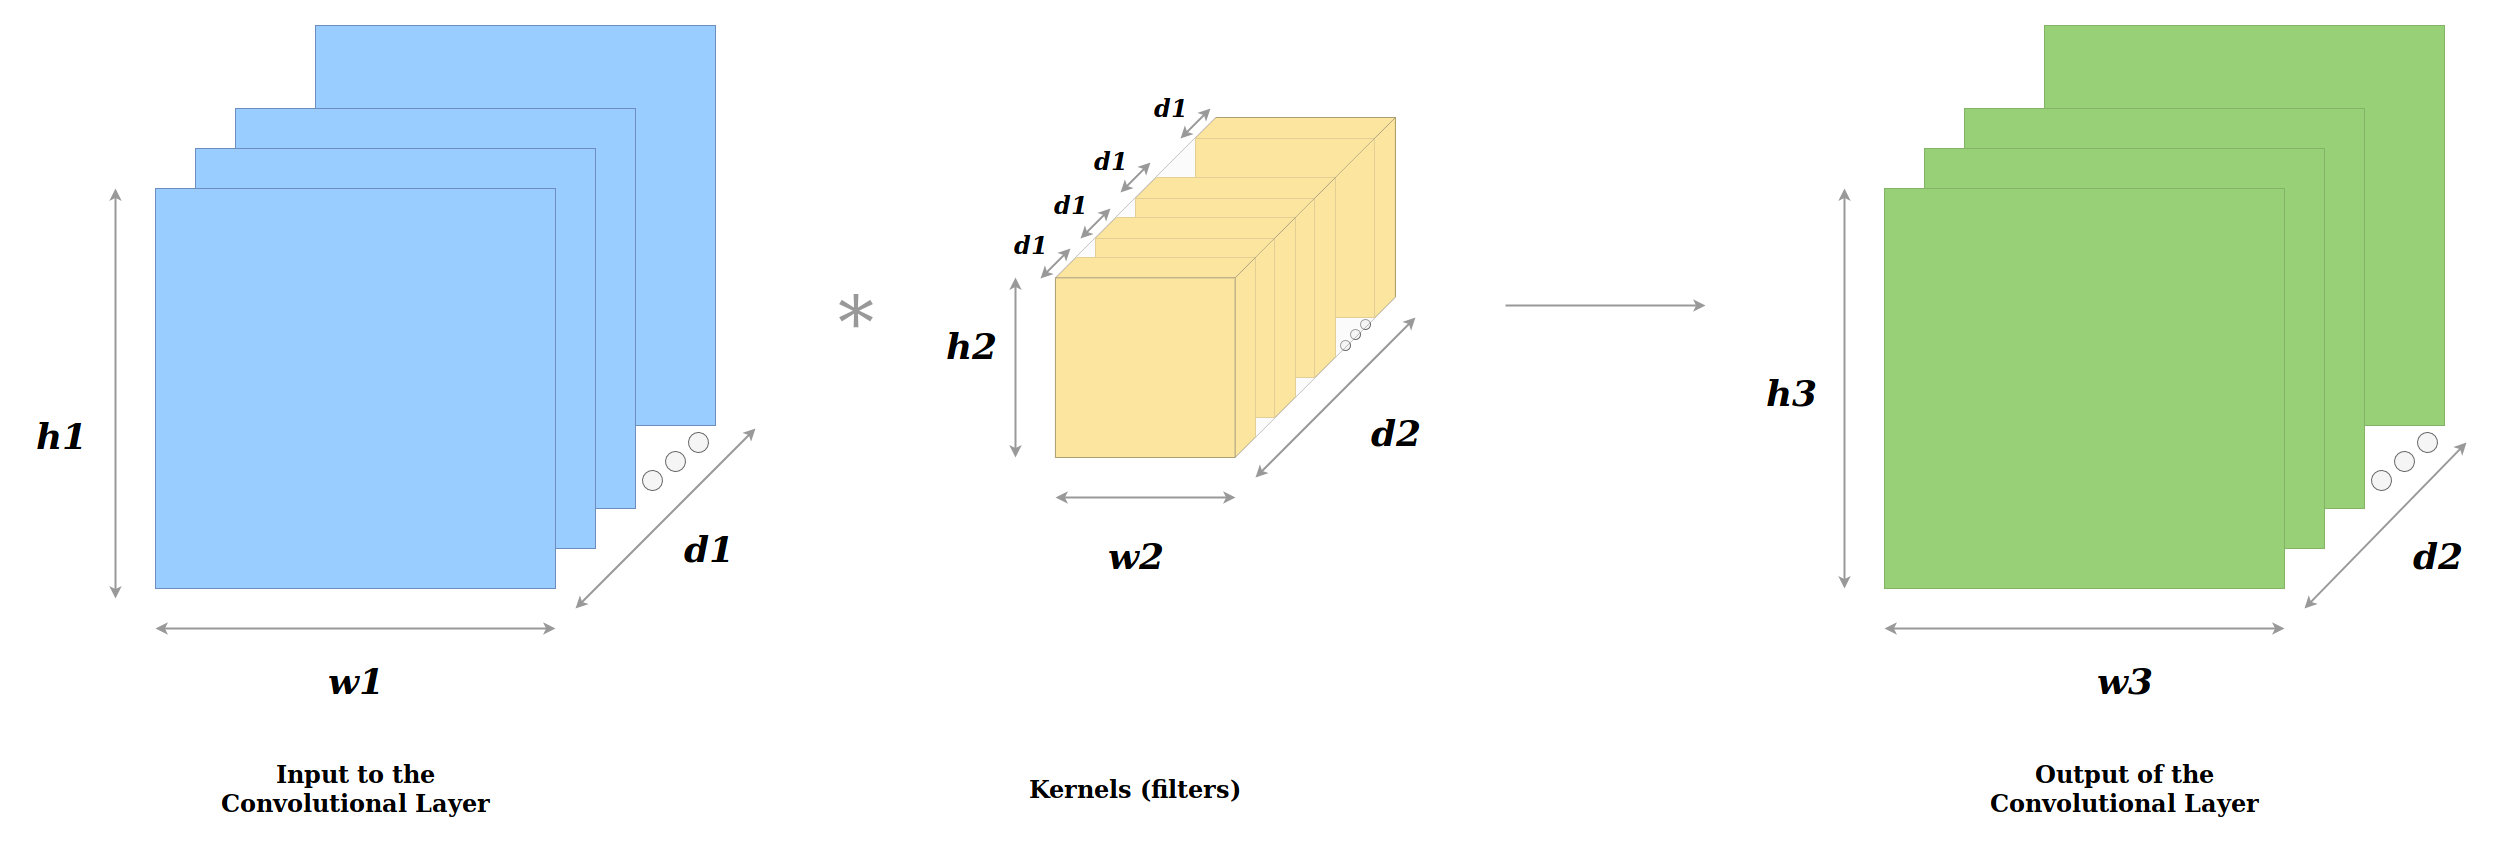
\includegraphics[width=4in]{../cap2_CNNs/src/conv2d.png}
    \caption{La convolución 2D puede ser usada con características de $d_1$ canales y devolver una característica de $d_2$ canales.} 
\end{figure}
 %------------------------------ Padding -----------------------
 \subsection{Padding}
 Debido a que la operación de convolución utiliza  pixeles adyacentes, no es posible calcular los bordes de la imagen resultante. Suponiendo que se tiene una imagen de $n\times n$ y un kernel de $k\times k$ con $k$ impar. Sólo es posible calcular la parte interior de la imagen resultante de tamaño $n-k+1$.
 \begin{figure}[H]
    \centering
     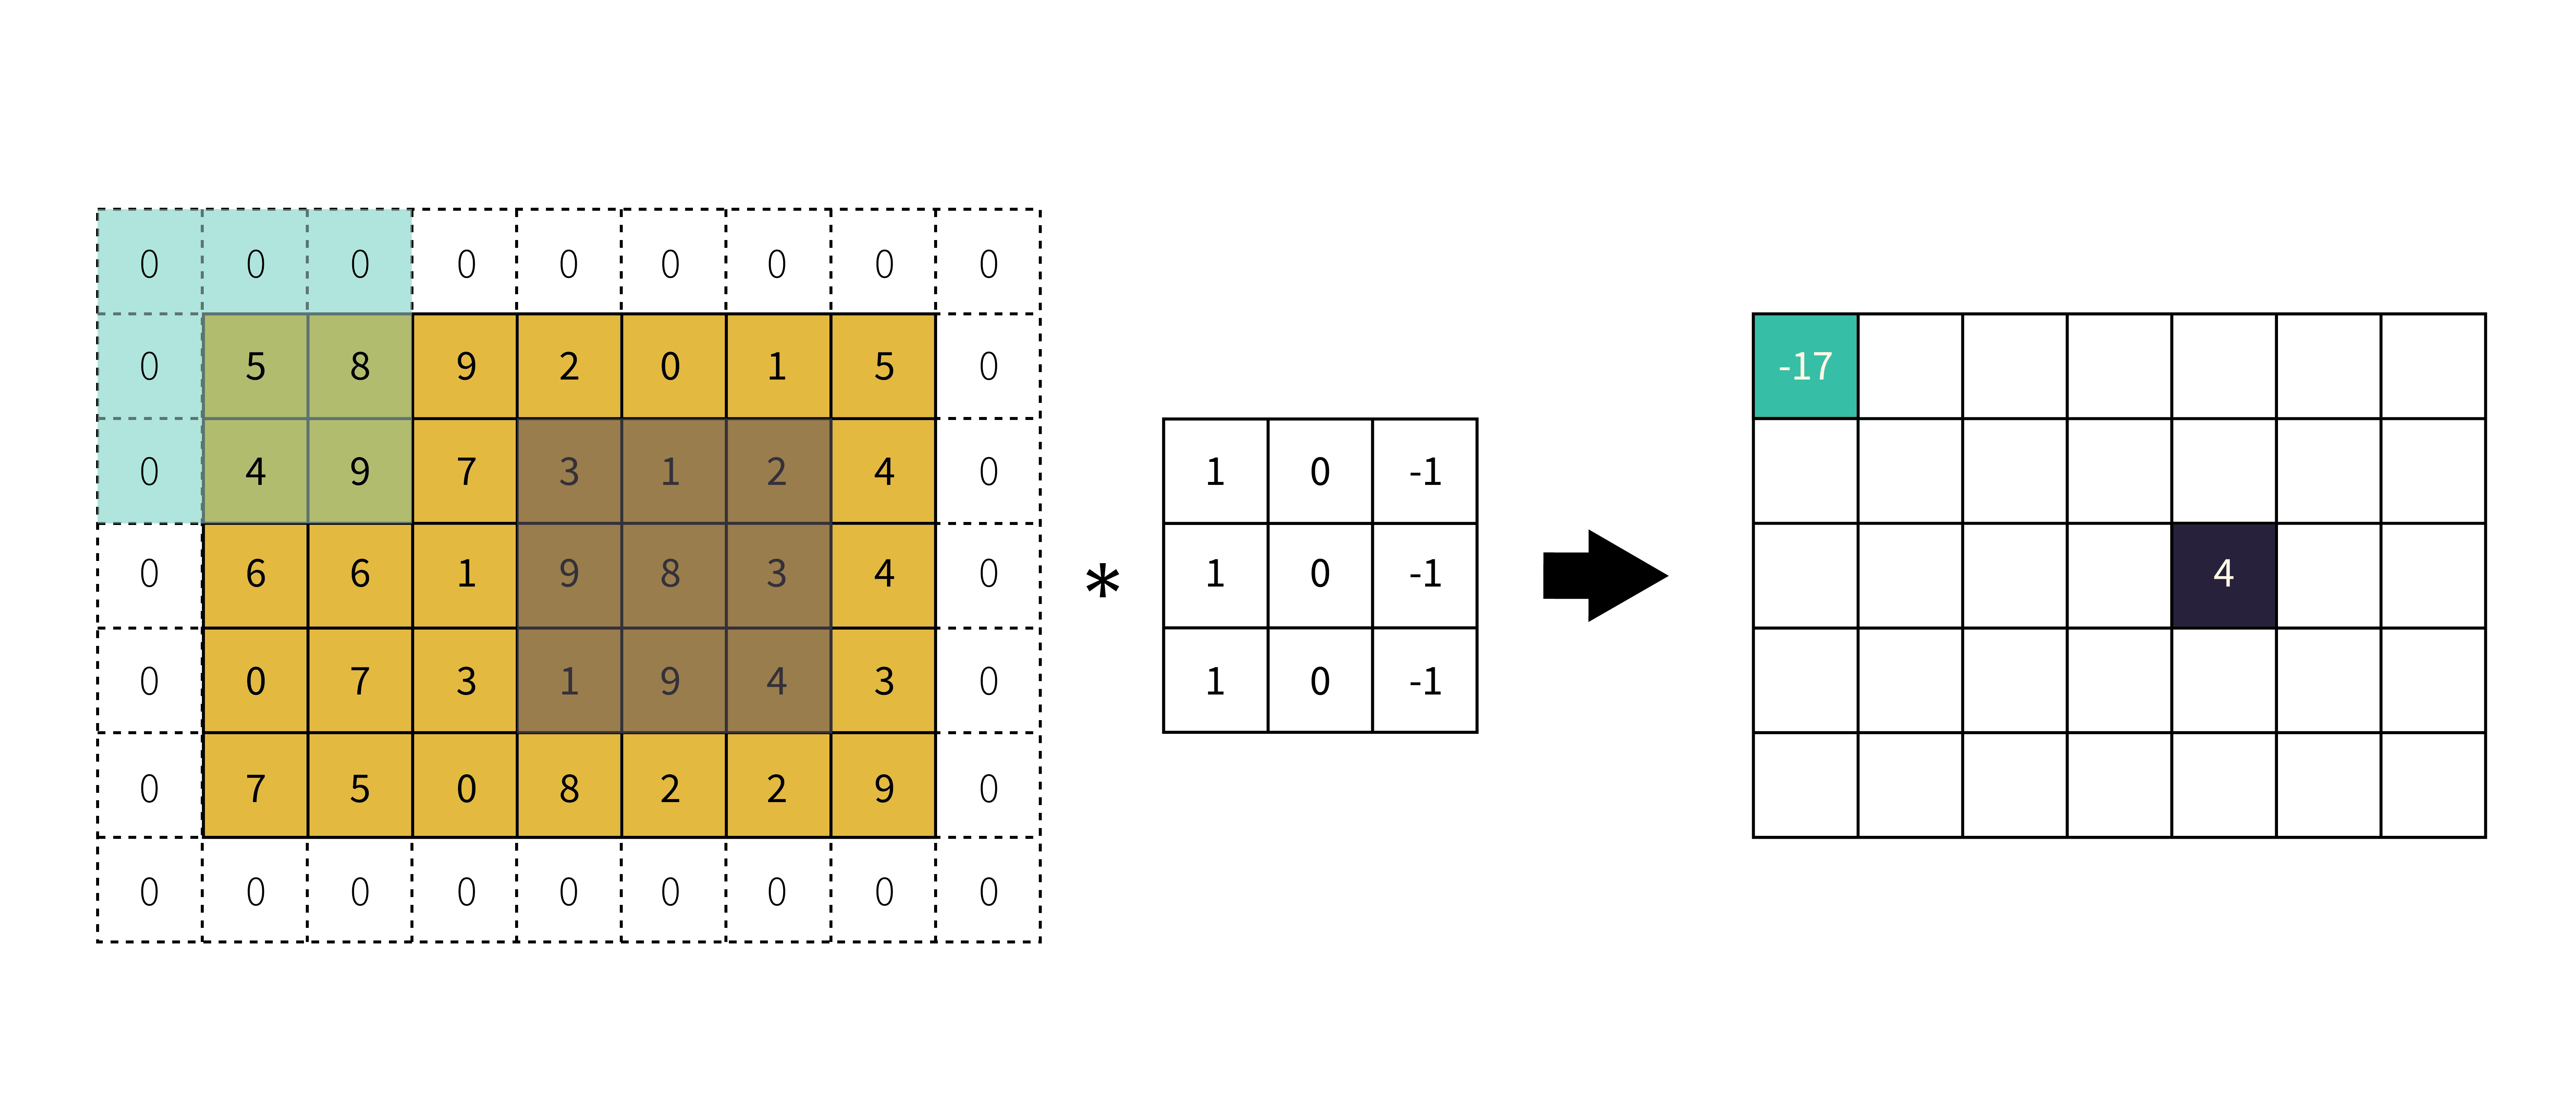
\includegraphics[width = 5in]{../cap2_CNNs/src/padding.png}
     \caption{\textcolor{red}{Usar una imagen propia}}
 \end{figure} 
 Para solucionar este problema, en vez de hacer la convolución con la imagen original $I$, extendemos la imagen hacia todos lados $\frac{k-1}{2}$ pixeles y realizamos una nueva convolución con la imagen extendida $\tilde I$.
 La nueva imagen $\tilde I$ contiene la misma información que la imagen original $I$, por tanto no importa la información que se añada en los nuevos pixeles. Sin embargo varias estrategias heurísticas han sido desarrolladas con el paso de los años:
\begin{itemize}
    \item \textcolor{red}{\textbf{Constant Padding.}} Cuando  se agrega un valor $c$ en todo el borde. Cuando $c = 0$ se conoce como \textcolor{red}{Zero Padding}.
    \item \textcolor{red}{\textbf{Zero Padding.}} Una posible opción y de las más utilizadas, es agregar ceros en el borde. En \cite{padding} se descubrió que utilizando este tipo de \textcolor{red}{padding} codifica cierto grado de información de las posiciones absolutas. Efecto que no ocurre cuando no se utiliza ningún tipo de \textcolor{red}{padding}. 
    \item \textcolor{red}{\textbf{Reflection Padding.}} Este padding se basa en reflejar los valores con respecto al borde \cite{type_of_paddings}.
    \item \textcolor{red}{\textbf{Symmetric Padding.}} Este padding es muy similar al \textcolor{red}{reflection padding}. En cada fila toma todos los valores y los invierte. Siendo esto lo que aparece en los bordes.
\end{itemize}
\begin{definition}
    Sea $x\in \mathbb R^{h\times w}$ una característica. Sea $\tilde x \in R^{(h+2s)\times (w+2r)}$ con $s < h$ y $r < w$ la característica extendida. Definimos algunos de los \textcolor{red}{paddings} como sigue: 
    \begin{enumerate}
        \item \textcolor{red}{Zero Padding}: 
        \begin{equation}           
            \tilde x_{i,j} = \left\{ 
                \begin{matrix}
                    x_{i-s, j-r} & \text{si} & s< i <h+s \quad \text{ y } \quad r< j < w+r \\
                    0 & \text{en otro caso}
                \end{matrix}
            \right..
        \end{equation}
        \item \textcolor{red}{Reflection Padding}:
        \begin{equation}           
            \tilde x_{i,j} = \left\{ 
                \begin{matrix}
                    x_{i-s, j-r} & \text{si} & s< i <h+s \quad \text{ y } \quad r< j < w+r \\
                    x_{i-s, r-j+2} & \text{si} & j < r \\
                    x_{s-i+2, j-r} & \text{si} & i < s \\
                    x_{2h+s-i, j-r} & \text{si} & i > h+s \\
                    x_{i-s, 2w+r-j} & \text{si} & j > w+r \\
                \end{matrix}
            \right..
        \end{equation}
    \end{enumerate}  
\end{definition}
En \cite{type_of_paddings} tras un estudio exhaustivo en el Image Net concluyen que el \textcolor{red}{symmetric padding} y el \textcolor{red}{reflection padding} obtienen peores resultados que el \textcolor{red}{Zero padding}. 
 %------------------------------ Pooling -----------------------
\subsection{Agrupación (Pooling)}
Una vez que la red encuentra características en una imagen, es posible que algunas secciones relevantes sean más grandes que otras. Por eso mismo, se implementa el \textcolor{red}{Downsampling}, es decir reducir el tamaño de las imágenes, para que nuestro kernel pueda encontrar cosas de distintos tamaños conforme las capas van reduciendo el tamaño de la imagen. La pregunta que surge es, ¿Cómo reducimos el tamaño de una imagen?  Sea como sea, siempre algo de información se pierde. Sin embargo existen métodos para resumir la información de varios pixeles en un sólo pixel. Algunos de estos métodos son
\begin{itemize}
    \item \textcolor{red}{\textbf{Max pooling}}. Dada una vecindad rectangular de pixeles, la \textcolor{red}{Max pooling} consiste en tomar el máximo valor dentro de esta vecindad. 
    \item \textcolor{red}{\textbf{Average pooling}}. Al igual que en el anterior caso, se toma una vecindad rectangular de pixeles. Sin embargo, en este caso se toma el promedio de todos los pixeles.
    \item \textbf{Un punto intermedio}. Considérese $v$ el vector de pixeles que debe reducirse a un sólo pixel . En \cite{pooling_analysis} se analiza el uso de diferentes agrupaciones, y se obtienen distintas parametrizaciones para hallar el valor del pixel $f_P(v)$ que sintetiza la información de $v$. Una posible parametrización es $f_P(v) = \left(\frac{1}{d}\sum_{i= 1}^{d}v_i^P\right)^{\frac{1}{P}}$. Donde $P=1$ es el \textcolor{red}{average pooling} y si $P\to \infty$ es el \textcolor{red}{max pooling}. Por tanto, es posible utilizar otros valores de $P$ para obtener \textcolor{red}{poolings} diferentes.
\end{itemize} 
\begin{figure}[H]
    \centering
    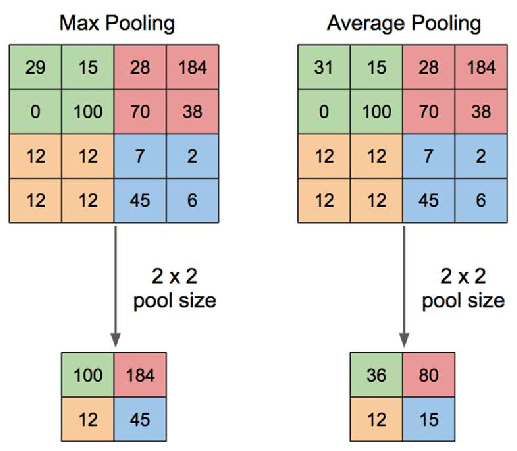
\includegraphics[width=4in]{../cap2_CNNs/src/pooling.png}
    \caption{\textsc{Ejemplo de maxpooling y averagepooling con regiones rectangulares de $2\times 2$.}} 
\end{figure}
También es posible en vez de hacer un \textcolor{red}{pooling} hacer una convolución con cierto tamaño de paso, con la intención de reducir el tamaño de la imagen. Esto no ha remplazado al \textcolor{red}{maxpooling} pero en la literatura se observan resultados prometedores. 
% ------------------------ Global pooling layers
\subsubsection{\textcolor{red}{Global pooling layers} }
Además de hacer un \textcolor{red}{downsampling}, también es común que en algún punto de la red, se reduzca una característica a un valor escalar, o en caso de una imagen con $d$ canales es posible obtener un vector en $\mathbb R^d$ \cite{CNNdefinition}.
\begin{definition}
    Sea $x\in \mathbb R^{h\times w}$ una característica. El operador \textcolor{red}{global average pooling}, $P_g: \mathbb R^{hw}\to \mathbb R$ se define como:
    \begin{equation}
        P_g(x) = \frac{1}{hw}\sum_{i=1}^h\sum_{j=1}^w x_{i,j}.
    \end{equation}
    Más aún, sea $x \in \mathbb R^{h\times w \times d}$ una característica. El operador \textcolor{red}{global average pooling}, $P_g: \mathbb R^{hw}\to \mathbb R$ se define como:
    \begin{equation}
        P_g(x) = (P_g(x_1), ..., P_g(x_d)).
    \end{equation}
\end{definition}
% ------------------------ Convolución como una operación lineal
\subsection{Convolución como una operación lineal}
 Es posible ver una convolución como una multiplicación por una matriz poco densa, en donde varios elementos de la matriz están restringidos a ser iguales a otros. Para las convoluciones de una variable, tiene que ser una \textsl{matriz de toeplitz}. En lo que refiere a dos dimensiones, una convolución es equivalente a una \textsl{Doble Matriz Circulante por Bloques} [Definición \ref{doubly_circulant_matrix}]. Es decir, se tiene lo siguiente 
 \begin{corollary}
    Sea $I$ una imagen, y $K$ un kernel. Existe una matriz $\hat K$ 
    \begin{equation}
        I*K = \text{vec}(I)\hat K.
    \end{equation}
 \end{corollary}

 %------------------------------ Redes Neuronales convolucionales -----------------------
\section{Redes Neuronales Convolucionales}
\label{section_cnn}
Consideremos el problema de clasificación. Sea $m$ la cantidad de clases posibles. Dados $y_1, y_2, ..., y_s \in \mathbb R^d$ y sus etiquetas $c_1, c_2, ..., c_s\in \mathbb R^m$, en donde la $k$-ésima entrada de $c_i$ puede ser $1$ o $0$. Cada vector $c_i$ tiene únicamente una entrada con valor $1$, que determina exactamente a que clase pertenece $y_i$.

    Sean 
    \begin{equation}
        \label{clasification}
        Y_0 = [y_1, y_2, ..., y_s]^T \quad \text{ y }, \quad  C = [c_1, ..., c_s]^T.
    \end{equation}

    El objetivo es poder clasificar correctamente datos no etiquetados. Para ello se han desarrollado diferentes arquitecturas de redes neuronales, y en el 2015 las Redes Neuronales Convolucionales obtuvieron el primer lugar en el concurso Image Net \cite{imageNet_dataset}, consiguiendo resultados sin precedenes \cite{resnet0}. 


 %------------- Descenso del gradiente
\subsection{Descenso del Gradiente Estocástico}
Ya que el problema de aprendizaje, es un problema de optimización, podemos recurrir a la teoría de optimización conocida. El algoritmo más común en el aprendizaje automático es el \textsl{descenso de gradiente estocástico} (SGD por sus siglas en inglés), el cuál es un algoritmo numérico para encontrar mínimos locales de una función. La intuición se basa en que si se tiene un punto $x\in D_f$, la dirección en dónde más decrece es $-\nabla f$. Éste método consiste en dos pasos
\begin{enumerate}
    \item Se selecciona un punto inicial $x_0$ en el dominio.
    \item Se actualiza nuestro valor $x_{i+1} = x_i - \alpha\nabla f(x_i)$ para $i = 1, ... N$
\end{enumerate}
donde $N$ es el número de iteraciones totales y $\alpha$ es un escalar, el cuál se conoce como razón de aprendizaje (learning rate). Es importante seleccionar una razón de aprendizaje apropiado, pues en caso de seleccionar una muy grande, el algoritmo podría diverger, por el contrario si se selecciona una muy pequeño, entonces el entrenamiento podría ser demasiado lento. 

Para calcular el gradiente de manera exacta, es necesario utilizar todo el conjunto de datos, lo cuál puede traducirse a tiempos elevados de cómputo. Es por eso, que en la práctica, se utiliza únicamente un subconjunto aleatorio de datos, calculando así, una aproximación al gradiente $\nabla J$ de la funcion de costo. Debido a este artificio que reduce el tiempo de entrenamiento, es que nuestro algoritmo es considerado estocástico.
\begin{figure}[H]
    \centering
    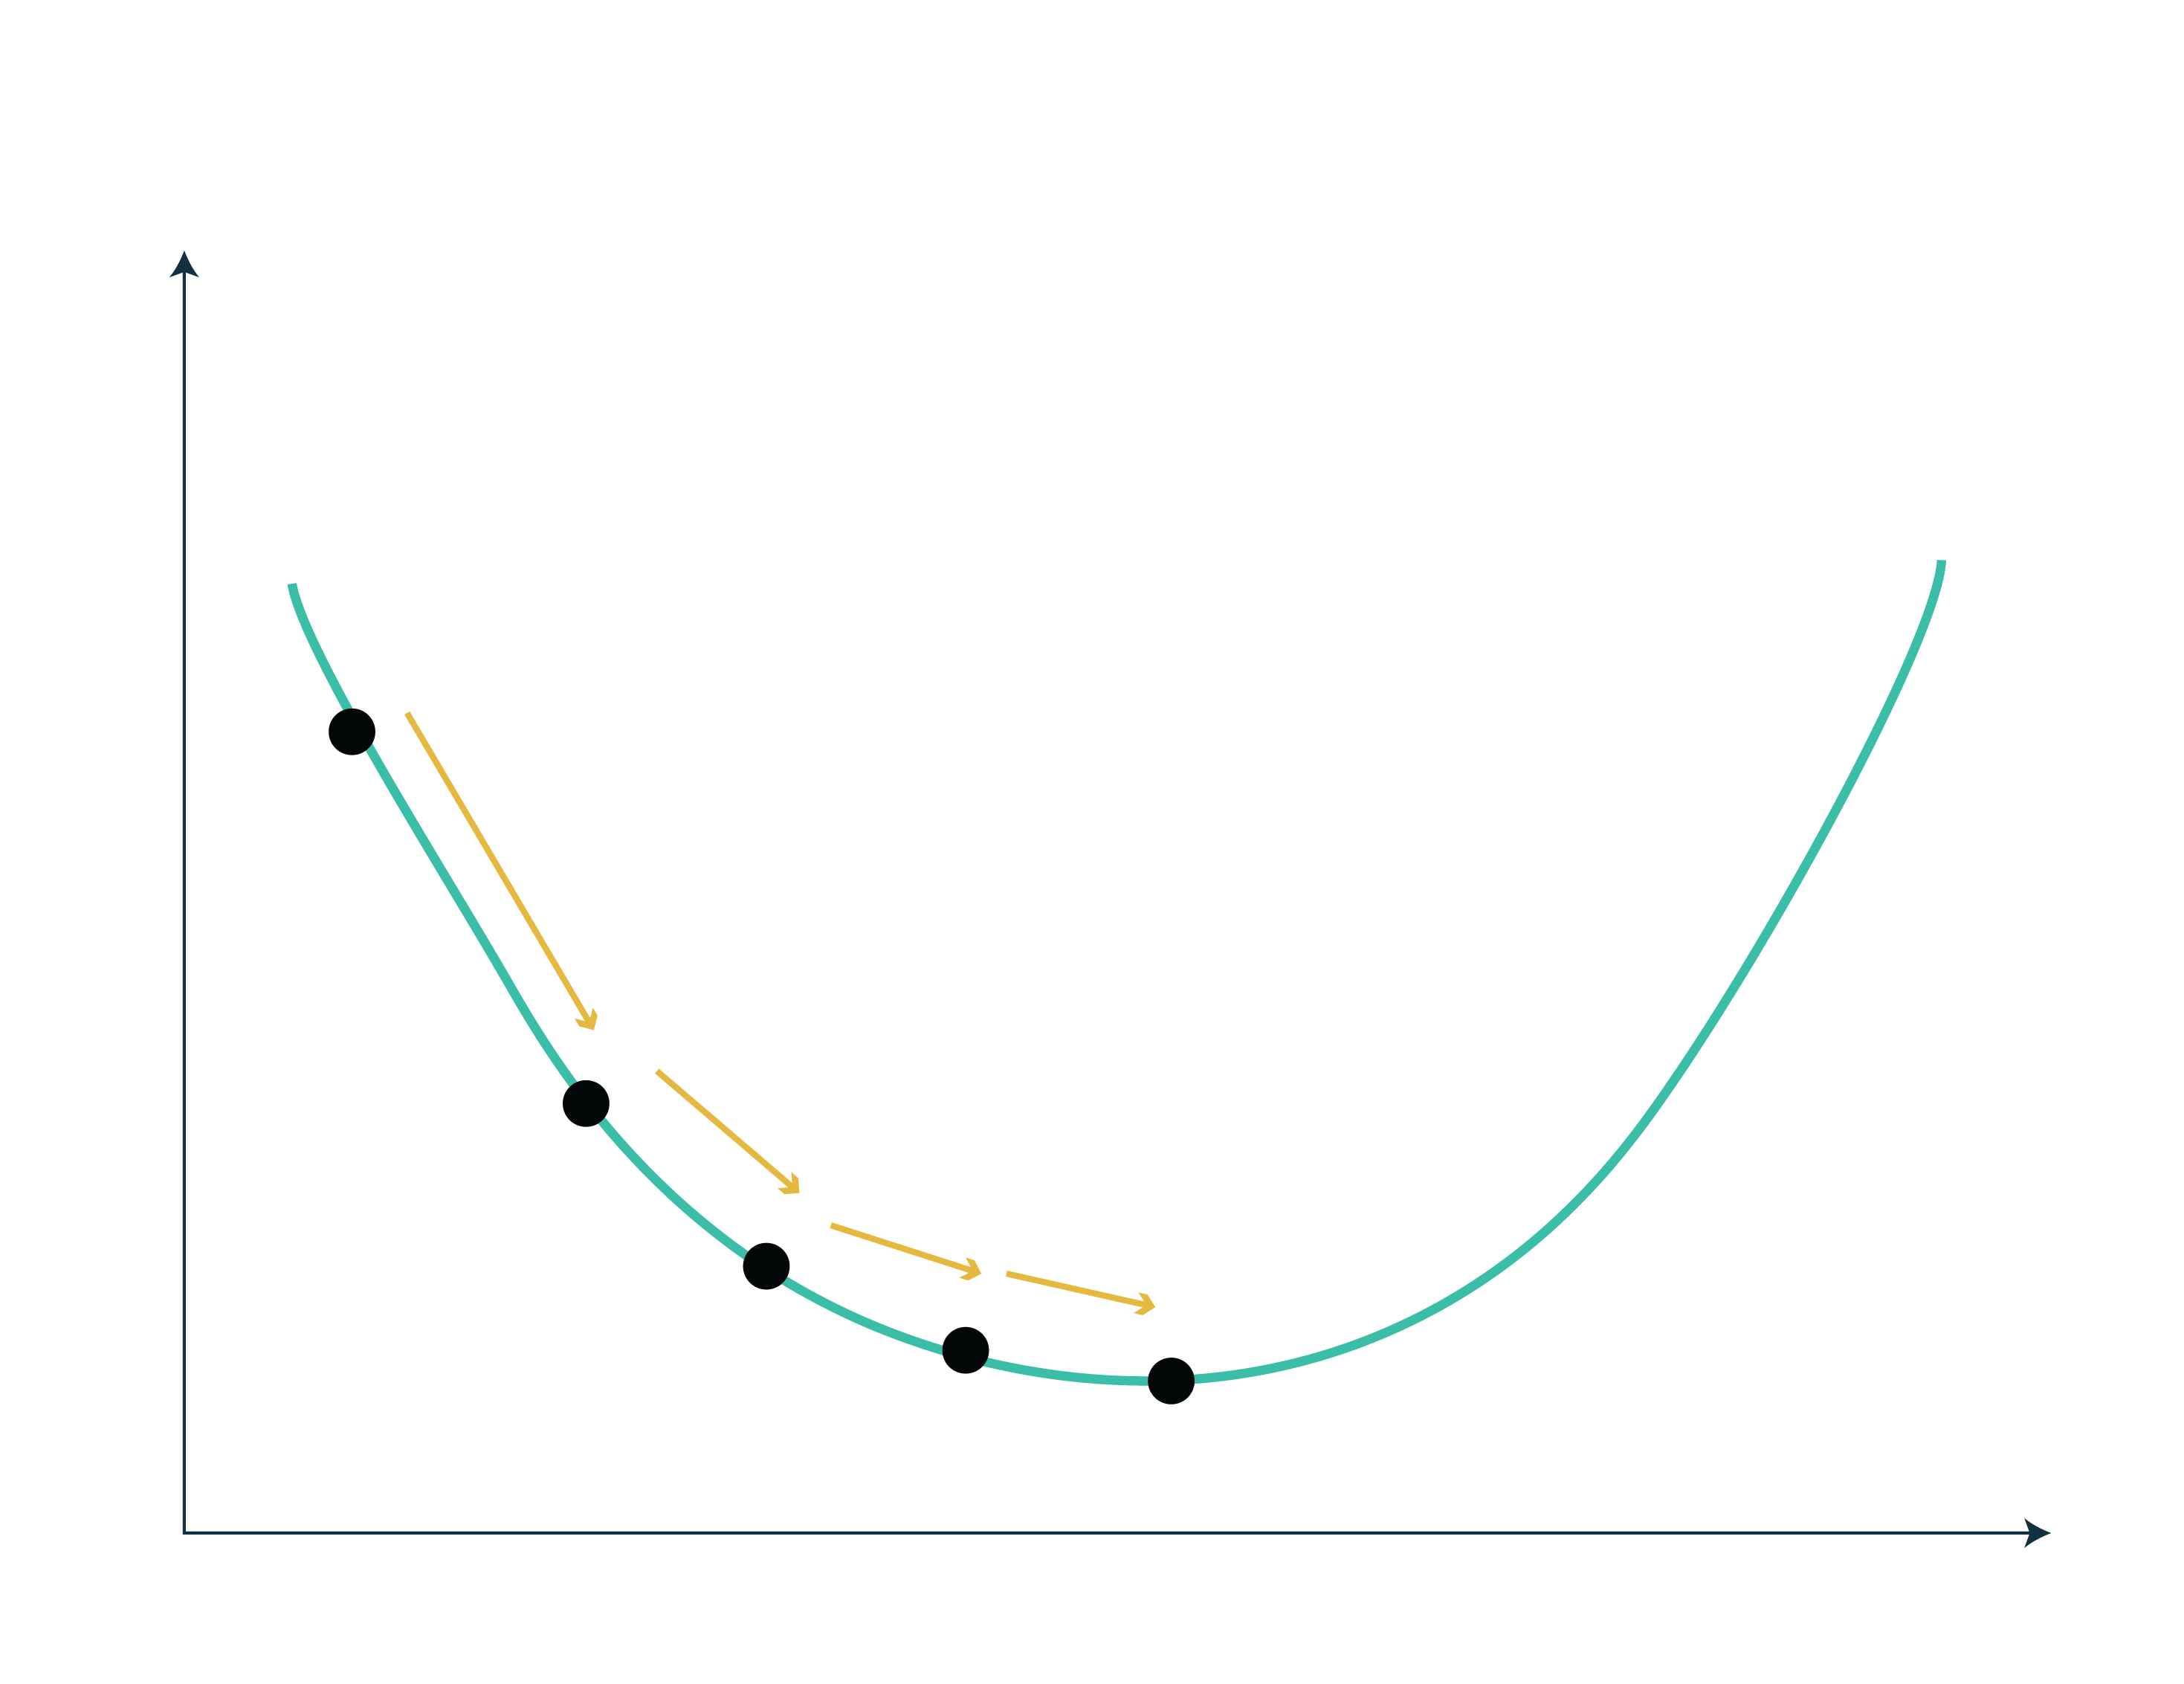
\includegraphics[width=4in]{../cap2_CNNs/src/sgd.png}
    \caption{\textcolor{red}{Seleccionar su propia imagen}} 
\end{figure}
\subsection{Optimizadores}
\label{subsection:optimizadores}
Existe una amplia literatura en el área de optimización de funciones. Por lo que es natural pensar que el SGD no es el único método para optimizar la función de costo. Debido a que la evaluación de dicha función, involucra millones de parámetros en las redes profundas actuales, no todos los algoritmos de optimización son adecuados para esta tarea. Aquí se presentan los métodos más efectivos investigados en los últimos años.

\subsubsection{AdaGrad}
A diferencia del SGD, el Algoritmo de Gradiente Adaptativo o AdaGrad \cite{adagrad}, actualiza la razón de aprendizaje con cada iteración. El algoritmo tiene un mejor desempeño en presencia de gradientes dispersos, es decir cuando el vector del gradiente contiene varios ceros.

\begin{equation}
    \theta_t = \theta_{t-1} - \frac{\alpha}{\sqrt{b_t} + \epsilon} g_{t-1}
\end{equation}
dónde $b_{t-1}$ es la suma del cuadrado de los gradientes.
\begin{equation}
    b_t = \sum_{i=1}^tg_{t-1}^2
\end{equation}

\subsubsection{RMSProp}
El algoritmo RMSProp fue propuesto por Geoff Hinton motivado en resolver el problema de las razones de aprendizaje sumamente pequeñas que se obtenían con el algoritmo AdaGrad y por consiguiente, evitar el desvanecimiento del gradiente.

\begin{equation}
    E[g^2]_t = \beta E[g^2]_{t-1} + (1-\beta)g_t^2
\end{equation}
\begin{equation}
    \theta_t = \theta_{t-1} - \frac{\alpha}{\sqrt{E[g^2]_t + \epsilon}}g_t
\end{equation}
\subsubsection{Adam}
El Estimador de momento Adaptativo (Adam por sus siglas en inglés) \cite{adam} se basa en momentos de primer y segundo orden del gradiente. Este método fue creado con la intención de obtener los beneficios de 2 optimizadores anteriores: el AdaGrad y el RMSProp. 


Para calcular los parámetros $\theta_t$, es necesario calcular el gradiente $g_t= \nabla f(\theta_{t-1})$. Denotamos  $m_t$ a la media movil exponencial, y $v_t$ al gradiente cuadrado. Los cuales se calculan de la siguiente manera:
\begin{equation}
    m_t = \beta_1 m_{t-1} + (1-\beta_1)g_t,
\end{equation}
\begin{equation}
    g_t = \beta_2 v_{t-1} + (1-\beta_2)g_t^2,
\end{equation}
dónde $\beta_1, \beta_2\in [0,1)$ son hiperparámetros que controlan el decrecimiento exponencial.

Los momentos $\hat m_t$ y $\hat v_t$ son la media y la varianza no centrada respectivamente.

\begin{equation}
    \hat m_t = \frac{m_t }{1-\beta_1^t},
\end{equation}
\begin{equation}
    \hat v_t = \frac{v_t}{1-\beta_2^t}.
\end{equation}

El optimizador Adam, actualiza los parámetros de la siguiente manera:
\begin{equation}
    \theta_t = \theta_{t-1} - \frac{\alpha \hat m_t}{\sqrt{\hat v_t} + \epsilon}.
\end{equation}
Dónde $\alpha$ es el tamaño de paso y $\epsilon$ es un valor cercano a cero.
\subsection{Propagación hacia atrás}
Ahora que se tiene un algoritmo para optimizar una función de costo, la pregunta natural es ¿Cómo obtenemos el gradiente? Siendo la propagación hacia adelante de una red, una función tan complicada y con tantos parámetros, es muy difícil calcular de manera analítica nuestro gradiente. Por buena suerte para nosotros, existe una técnica conocida como \textsl{propagación hacia atrás}, encargada de calcular numéricamente el gradiente de la función de costo.


\subsection{Normalización por Lotes}
Entre las téncicas de regularización más utilizadas se encuentra la \textsl{normalización por lotes} (BN por sus siglas en inglés). En el 2015 en un artículo de google \cite{batchNormalization} se describe esta técnica y se constata que tiene múltiples beneficios tales como incrementar la razón de aprendizaje, conseguir que el entrenamiento sea más independiente de la inicialización y además actuar como regularizador.

\begin{definition}
    Sea $\mathcal{B} = \{x^{(1)}, x^{(2)}, \ddots, x^{(m)}\}$ un lote de características. La normalización por lotes de $\mathcal B$ se define como:
    \begin{equation}
        B(x^{(i)}; \gamma, \beta) := \frac{\gamma(x^{(i) - \mu})}{\sigma} + \beta, \quad i=1,2...,m,
    \end{equation}
    donde  $\mu := \sum^m_{i=1}x^{(i)}/m$ y $\sigma^2 = \sum^m_{i=1}(x^{(i)}-\mu)^2/m$.
\end{definition}
Los parámetros $\gamma$ y $\beta$ usualmente se aprenden en la optimización. Cuando se usa la normalización por lotes, no es necesario agregar \textcolor{red}{biases} pues son calculados explícitamente a través de $\beta$.

Ahora que conocemos lo que es una convolución, se define matemáticamente una Red Neuronal Convolucional.   
\begin{definition} 
    Sea $x_0\in \mathbb R^{h\times w\times d}$ una característica. La propagación hacia adelante de una CNN está determinada por el siguiente esquema recursivo

    \begin{equation}
        x_{n+1} = \sigma(x_n * K_n + b_n).
    \end{equation}
    donde $\sigma$ es una función de activación, $K_n$ representa un Kernel y $b_n\in \mathbb R^d$ es el \textcolor{blue}{bias}.
\end{definition}
En las primeras arquitecturas sea usaban Redes Completamente Conectadas (FCN por sus siglas en inglés) tal como se aprecia en la Figura \ref{cnn_example_img}. Sin embargo en los últimos años se ha visto un incremento en el uso de Redes Completamente Convolucionales.

\begin{figure}[H]
    \centering
    
    \includegraphics[width=5in]{../cap2_CNNs/src/convolution_arquitecture.png}
    \caption{\label{cnn_example_img} Ejemplo de arquitectura de una Red Neuronal Convolucional. En la figura se aprecia la imagen de entrada, las capas convolucionales y la FCN que determina la clase \cite{image:cnn}} 

\end{figure}


\subsection{Desvanecimiento del gradiente}
Los mayoría de los algoritmos de optimización, dependen del gradiente. Y los algoritmos que utilizan la propagación hacia atrás, en ocasiones presentan el problema conocido como \textsl{desvanecimiento del gradiente}, que consiste en que los gradientes se vuelven tan pequeños que previenen al modelo de continuar con el proceso de aprendizaje.

\subsection{CNNs en el Estado del Arte}
En 2012 en el ImageNet ocurrió algo sin precedentes en dicha competencia. El ganador del concurso se había llevado el primer lugar absoluto, obteniendo una ventaja de 10.9$\%$ de error por debajo del segundo lugar. Es así como la \textsl{AlexNet} \cite{alexnet} consiguió reputación para las CNNs. Para 2013, la red ganadora del ImageNet(2013) fue la Zf-net \cite{zfnet}, la cuál era una modificación de los hiperparámetros de la AlexNet.

\begin{figure}[H]
    \centering
    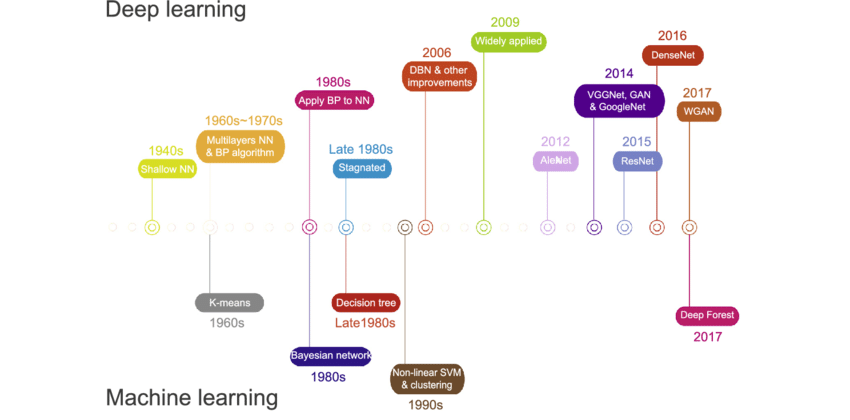
\includegraphics[width=5in]{../cap2_CNNs/src/timeline.png}
    \caption{Línea de tiempo de las Redes en el Estado del Arte} 
\end{figure}
 %------------------------------ ResNet -----------------------
\section{ResNet}
\label{resnet_section}
Las \textsl{Redes Neuronales Residuales} fueron presentadas en 2015 por Kaiming He et. al. en \cite{resnet0}. Uno de los mayores retos en el diseño de redes profundas, es el \textsl{desvanecimiento del gradiente}. Es decir, por la naturaleza de la propagación hacia atrás, las redes muy profundas, implican el cálculo de gradientes con entradas muy pequeñas, y eventualmente el gradiente se desvanece y previende el aprendizaje de la red.
Es decir, $\|\nabla_\theta L\| = 0$ dónde $L$ es la función de pérdida y $\theta$ son los parámetros. 

Antes del 2015 existían dificultades para alcanzar redes con profundidades mayores a 20 capas. Para solucionar este problema, se crearon las \textsl{conexiones de salto}.

\begin{definition} 
    Consideremos el problema de clasificación (\ref{clasification}). Sea $x_0\in \mathbb R^h\times w\times d$ una característica. La propagación hacia adelante de la ResNet está determinada por el siguiente esquema recursivo 

    \begin{equation}
        \label{resnet_equation}
        x_{n+1} = x_n + \sigma(x_n * K_n + b_n).
    \end{equation}
    donde $\sigma$ es una función de activación, $K_n$ representa un Kernel y $b_n\in \mathbb R^d$ es el \textcolor{blue}{bias}.
\end{definition}
Ya que la operación de convolución puede ser expresada como una multiplicación de matrices, es posible reescribir la ecuación (\ref{resnet_equation}) como:
\begin{equation}
    \label{resnet_equation_modified}
    X_{n+1} = X_n + \sigma(X_nA_n + b_n).
\end{equation}
dónde $X_0 = \vect{x_0}$ y $A_n$ es la matriz que induce el kernel $K_n$. 

La diferencia entre una CNN convencional es el término $X_n$ que se agrega a $\sigma(\cdot)$, conocida como conexión de salto, cuyo propósito es estabilizar el gradiente, para evitar su explosión o desvanecimiento.

\begin{figure}[H]
    \centering
    
    \includegraphics[height=3in]{../cap2_CNNs/src/resnet_block.png}
    \caption{Diagrama de un bloque de ResNnet.} 

\end{figure}

Pese a que la ecuación (\ref{resnet_equation_modified}) es la forma canónica de definir una ResNet, también es posible usar otras funciones en vez de sólo la composición de la función de activación con una función lineal. Por lo que una definición más general de la ResNet es
\begin{equation}
    X_{n+1} = X_n + F_n(X_n) 
\end{equation}

En la ResNet original se observa que $F_n(x) = \sigma(xA_n + b_n)$. Sin embargo se han usado otras funciones. En \cite{DBLP:journals/corr/abs-1806-03751} se toma 
\begin{equation}
    \label{resnet_block_function}
    F_n(x) = \text{BN}(\hat K_n *\text{ReLU}(\text{BN}(K_n * x)))
\end{equation}
que en la versión de multiplicación de matrices es:
\begin{equation}
    F_n(x) = \text{BN}(\text{ReLU}(\text{BN}(x \cdot A_n)) \cdot B_n),
\end{equation}
dónde $A_n$ y $B_n$ son las matrices correspondientes a los filtros $K_n$ y $\hat K_n$ de manera respectiva, BN y ReLU son las funciones de Normalización por lotes y Unión lineal Rectificada y la operación $M\cdot N$ es la multiplicación de matrices convencional colocada para mayor claridad.  

La función (\ref{resnet_block_function}) es también la utilizada en la biblioteca de pyTorch \cite{pytorch_library} en el repositorio:\\
\\
\url{https://github.com/pytorch/vision/blob/main/torchvision/models/resnet.py}. \\
\\
Además de los bloques con conexiones de salto, las arquitecturas modernas cuentan con otras capas, incluyendo capas convolucionales, normalizaciones e incluso una Red Completamente Conectada (FCN por sus siglas en inglés) en la parte final de la propagación. Una de las ResNet más populares, es la ResNet-50


\begin{figure}[H]
    \centering
    \includegraphics[width=4in]{../cap2_CNNs/src/resnet50.png}
    \caption{Diagrama de una ResNet-50} 
\end{figure}
%------------- Estabilidad de las redes neuronales
\subsection{Inicialización de parámetros}
Los algoritmos de optimización (Sección \ref{subsection:optimizadores}) requieren de un valor inicial $\theta_0$. En la mayoría de los casos, una selección adecuada de $\theta_0$ puede conseguir que el número de iteraciones se reduzca en comparación con un $\theta_0$ arbitrario. El Artículo \cite{weight_initialization} contiene un análisis dedicado a la inicialización de parámetros para aprendizaje profundo.

\subsubsection{Inicialización con Ceros}
Inicializar los parámetros con ceros es un acercamiento natural. Sin embargo, es conocido que si dos parámetros con la misma función de activación, están conectados con la misma entrada, entonces se modificarán de igual forma en el proceso de entrenamiento. De modo que se dice que la inicialización deber \textsl{romper la simetría} \cite{deeplearningbook}. El caso de la inicialización con ceros, o con cualquier constante, no satisface esta propiedad, por lo que no es recomendable usarlas.
\subsubsection{Inicialización Aleatoria}
Una manera sencilla de romper la simetría es  inicializando los parámetros de manera aleatoria. Una heurística común es inicializar la matriz de pesos $W$ con una distribución uniforme
\begin{equation}
    W_{i,j} = U\left(-\frac{1}{\sqrt{m}}, \frac{1}{\sqrt{m}}\right),
\end{equation}
donde $m$ es la cantidad de entradas, y $U[-a,a]$ la distribución uniforme de $-a$ hasta $a$. Sin embargo, al no prestar atención al comportamiento de los gradientes, esta forma de inicializar nuestros parámetros puede provocar desvanecimiento o  explosión del gradiente.
\subsubsection{Inicialización de Glorot}
Para \textsl{Inicialización de Glorot}, también conocida como la \textsl{inicialización de Xavier} \cite{glorot_initialization} se asume que los pesos son inicializados independientemente y que las varianzas de las características de entrada son iguales. Además se pretende que las varianzas de los gradientes en todas las capas sean iguales. Para ello se propone la siguiente inicialización :
\begin{equation}
    W_{i,j} \sim U\left(-\sqrt{\frac{6}{m+n}}, \sqrt{\frac{6}{m+n}}\right)
\end{equation}
donde se tienen $m$ valores de entrada y $n$ valores de salida.

\subsubsection{Inicialización con Kaiming}
La \textsl{inicialización de Kaiming} o \textsl{Inicialización de He} \cite{kaiming} asume funciones de activación del tipo Rectificador, tales como la ReLu o la PReLU. 
\begin{equation}
    W_l \sim \mathcal{N} \left(0, \frac{2}{n^l}  \right)
\end{equation}
dónde $n_l$ es la cantidad de elementos en la capa l.

 %------------- Estabilidad de las redes neuronales
\subsection{Estabilidad en las redes Neuronales}
\label{resnet_stability_introduction}
En clasificación de imágenes, una red debe ser robusta contra el ruido, o pequeñas modificaciones en la imagen.  En el artículo \cite{CNNdefinition} se establecen definiciones formales de estabilidad, cuyo principio básico es que la salida debe ser continua con respecto a la entrada.

\begin{definition}
    Supóngase $f$ la propagación hacia adelante de una red neuronal. Sea $x$ una imagen y $\hat x$ la misma imagen perturbada. Decimos que $f$ es estable con respecto a epsilon cuando 
    \begin{equation}
        \|f(x)-f(\hat x)\| < \epsilon
    \end{equation}
\end{definition}
En la práctica se pretende reducir lo más posible el valor de $\epsilon$. En \cite{stable_resnets} se agrega un término $h\in \mathbb R$ a la ResNet con la intención de añadirle estabilidad a la red
\begin{equation}
    X_{n+1} = X_n + h\sigma(X_nA_n + b_n).
\end{equation}